\section{Additional Theory}
\label{sec:additional-theory}

\subsection{Solution to the Elastic Net}%
\label{sec:elastic-net-estimator}

Let \((\hat{\beta}_0^{(n)}, \hat{\vec{\beta}}^{(n)})\) be a solution to the problem in
\Cref{eq:elastic-net}. Expanding \(f\) in \Cref{eq:elastic-net}, we have
\[
  \begin{aligned}
     & \frac{1}{2}\left( \vec y^\T \vec y - 2(\tilde{\mat{X}}\vec{\beta} + \beta_0)^\T\vec{y} + (\tilde{\mat{X}}\vec{\beta} + \beta_0)^\T(\tilde{\mat{X}}\vec{\beta} + \beta_0)\right) \\
     & + \lambda_1 \lVert \vec\beta \rVert_1 + \frac{\lambda_2}{2}\lVert \vec \beta \rVert_2^2.
  \end{aligned}
\]
Taking the subdifferential with respect to \(\vec{\beta}\) and \(\beta_0\), the KKT
stationarity condition yields the following system of equations:
\begin{equation}
  \label{eq:kkt-elasticnet}
  \begin{cases}
    \tilde{\mat{X}}^\T(\tilde{\mat{X}}\vec{\beta} + \beta_0 - \vec{y}) + \lambda_1 g + \lambda_2 \vec\beta \ni \vec{0}, \\
    n \beta_0 + (\tilde{\mat{X}}\vec{\beta})^\T \vec{1} - \vec{y}^\T \vec{1} = 0,
  \end{cases}
\end{equation}
where \(g\) is a subgradient of the \(\ell_1\) norm that has elements \(g_i\) such that
\[
  g_i \in
  \begin{cases}
    \{\sign{\beta_i}\} & \text{if } \beta_i \neq 0, \\
    [-1, 1]            & \text{otherwise}.
  \end{cases}
\]

\subsubsection{Orthogonal Features}

If the features of the normalized design matrix are orthogonal, that is,
\(\tilde{\mat{X}}^\intercal \tilde{\mat{X}} = \diag\left(\tilde{\vec{x}}_1^\T
\tilde{\vec{x}}_1, \dots, \tilde{\vec{x}}_p^\intercal \tilde{\vec{x}}_p\right) \), then
\Cref{eq:kkt-elasticnet} can be decomposed into a set of \(p + 1\) conditions:
%
\[
  \begin{cases}
    \tilde{\vec{x}}_j^\T (\tilde{\vec{x}}_j \beta_j + \ones \beta_0 - \vec{y}) + \lambda_2 \beta_j + \lambda_1 g \ni 0, & j \in [p], \\
    n \beta_0 + (\tilde{\mat{X}}\vec{\beta})^\T \vec{1} -  \vec{y}^\T \ones = 0.
  \end{cases}
\]
%
The inclusion of the intercept ensures that the locations (means) of the features do not
affect the solution (except for the intercept itself). We will therefore from now on assume
that the features are mean-centered so that \(c_j = \bar{\vec{x}}_j\) for all \(j\) and
therefore \(\tilde{\vec{x}}_j^\T \ones = 0\). A solution to the system of equations is then
given by the following set of equations~\citep{donoho1994}:
%
\begin{equation*}
  \label{eq:orthogonal-solution-normalized}
  \hat{\beta}^{(n)}_j = \frac{\st_{\lambda_1}\left(\tilde{\vec{x}}_j^\T \vec{y}\right)}{\tilde{\vec{x}}_j^\T \tilde{\vec{x}}_j + \lambda_2},
  \qquad
  \hat{\beta}_0^{(n)} = \frac{\vec{y}^\T \ones}{n},
\end{equation*}
%
where \(\st_\lambda(z) = \sign(z) \max(|z| - \lambda, 0)\) is the soft-thresholding
operator.

\subsection{Why Maximum--Absolute and Min--Max Scaling are Unsuitable for Normally Distributed Data}%
\label{sec:maxabs-theory}

In \Cref{thm:maxabs-gev}, we show that the scaling factor in the max--abs method converges
in distribution to a Gumbel distribution.

\begin{theorem}
  \label{thm:maxabs-gev}
  Let \(X_1, X_2, \dots, X_n\) be a sample of normally distributed random variables, each with mean \(\mu\) and standard deviation \(\sigma\). Then
  \[
    \lim_{n \rightarrow \infty}\Pr\left(\max_{i \in [n]} |X_i| \leq x\right) = G(x),
  \]
  where \(G\) is the cumulative distribution function of a Gumbel distribution with
  parameters
  \[
    b_n = F_Y^{-1}(1 - 1/n)\quad \text{and} \quad a_n = \frac{1}{n f_Y(\mu_n)},
  \]
  where \(f_Y\) and \(F_Y^{-1}\) are the probability distribution function and quantile
  function, respectively, of a folded normal distribution with mean \(\mu\) and standard
  deviation \(\sigma\).
\end{theorem}

The gist of \Cref{thm:maxabs-gev} is that the limiting distribution of \(\max_{i \in
  [n]}|X_i|\) has expected value \(b_n + \gamma a_n\), where \(\gamma\) is the
Euler-Mascheroni constant. This indicates that the scaling factor strongly dependent on the
sample size. In \Cref{fig:maxabs-gev}, we observe empirically that the limiting
distribution agrees well with the empirical distribution in expected value even for small
values of \(n\).

In \Cref{fig:maxabs-n} we show the effect of increasing the number of observations, \(n\),
in a two-feature lasso model with max-abs normalization applied to both features. The
coefficient corresponding to the Normally distributed feature shrinks as the number of
observation \(n\) increases. Since the expected value of the Gumbel distribution diverges
with \(n\), this means that there's always a large enough \(n\) to force the coefficient in
a lasso problem to zero with high probability.

\begin{figure}[htpb]
  \centering
  \subfigure[Theoretical versus empirical distribution of the maximum absolute value of normally distributed random variables.\label{fig:maxabs-gev}]{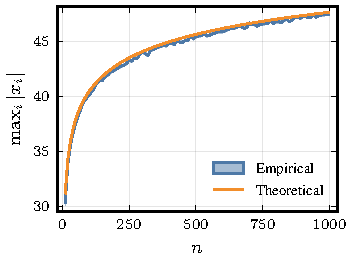
\includegraphics[]{plots/maxabs_gev.pdf}}%
  \hspace{1cm}
  \subfigure[Estimation of mixed features under maximum absolute value scaling\label{fig:maxabs-n}]{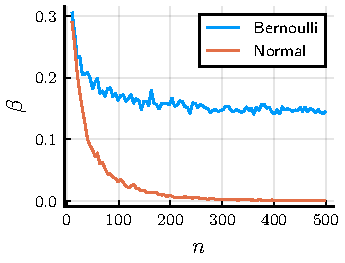
\includegraphics[]{plots/maxabs_n.pdf}}
  \caption{%
    Effects of maximum absolute value scaling
  }
\end{figure}

For min--max scaling, the situation is similar and we omit the details here. The main point
is that the scaling factor is strongly dependent on the sample size, which makes it
unsuitable for normally distributed data in several situations, such as on-line learning
(where sample size changes over time) or model validation with uneven data splits.

\subsection{Derivation of Bias and Variance of the Elastic Net Estimator}
\label{sec:bias-var-deriv}

Here, we derive the results in \Cref{sec:theory} in more detail. We have
\[
  {Z_j} = \tilde{\vec{x}}_j^\T \vec{y} = \tilde{\vec{x}}_j^\T(\mat{X}\vec{\beta}^* + \vec{\varepsilon}) = \tilde{\vec{x}}_j^\T (\vec{x}_j\beta_j^* + \boldsymbol{\varepsilon})
  \qquad
  \text{and}
  \qquad
  d_j = s_j(\tilde{\vec{x}}_j^\T \tilde{\vec{x}}_j + \lambda_2)
\]
so that \(\hat{\beta}_j = \st_{\lambda_1}({Z_j})/d_j\). Since \(d_j\) is fixed under our
assumptions, we focus on \(S_{\lambda_1}({Z_j})\). First observe that since \(c_j =
\bar{\bm{x}}_j\),
\[
  \begin{aligned}
    \tilde{\vec{x}}_j^\T \tilde{\vec{x}}_j & = \frac{1}{s_j^2}(\vec{x}_j - c_j)^\T (\vec{x}_j - c_j) = \frac{\vec{x}_j^\T\vec{x}_j - nc_j^2}{s^2_j} = \frac{n \nu_j}{s_j^2}, \\
    \tilde{\vec{x}}_j^\T \vec{x}_j         & = \frac{1}{s_j}(\vec{x}_j^\T \vec{x}_j - \vec{x}_j^\T \ones c_j) = \frac{n \nu_j}{s_j},
  \end{aligned}
\]
where \(\nu_j\) is the uncorrected sample variance of \(\vec{x}_j\). This means that
\begin{equation}
  {Z_j} = \frac{\beta_j^* n \nu_j- \vec{x}_j^\T \vec{\varepsilon}}{s_j}
  \qquad\text{and}\qquad
  d_j = s_j\left(\frac{n \nu_j}{s_j^2} + \lambda_2\right).
\end{equation}
For the expected value and variance of \({Z_j}\) we then have
\begin{align*}
  \E {Z_j}   & = \mu_j = \E \left( \tilde{\vec{x}}_j^\T (\vec{x}_j\beta^*_j + \vec{\varepsilon}) \right)  = \tilde{\vec{x}}_j^\T\vec{x}_j \beta^*_j = \frac{\beta_j^* n \nu_j}{s_j},            \\
  \var {Z_j} & = \sigma_j^2 = \var\left(\tilde{\vec{x}}_j ^\T \vec{\varepsilon}\right) = \tilde{\vec{x}}_j^\T \tilde{\vec{x}}_j\sigma_\varepsilon^2 = \frac{n\nu_j\sigma_\varepsilon^2}{s_j^2}.
\end{align*}

The expected value of the soft-thresholding estimator is
\begin{equation*}
  \E \st_\lambda({Z_j}) = \int_{-\infty}^\infty \st_\lambda(z) f_{Z_j}(z) \du z
  = \int_{-\infty}^{-\lambda}(z + \lambda)f_{Z_j}(z) \du z + \int_{\lambda}^\infty (z - \lambda)f_{Z_j}(z) \du z.
\end{equation*}
And then the bias of \(\hat\beta_j\) with respect to the true coefficient \(\beta_j^*\) is
\begin{equation*}
  \E \hat\beta_j - \beta_j^* = \frac{1}{d_j}\E \st_\lambda({Z_j}) - \beta^*_j.
\end{equation*}

Finally, we note that the variance of the soft-thresholding estimator is
\begin{equation}
  % \label{eq:st-variance}
  \var {S_\lambda({Z_j})} = \int_{-\infty}^{-\lambda}(z + \lambda)^2f_{Z_j}(z) \du z + \int_{\lambda}^\infty (z - \lambda)^2 f_{Z_j}(z) \du z - \left(\E \st_\lambda({Z_j})\right)^2
\end{equation}
and that the variance of the elastic net estimator is therefore
\begin{equation*}
  \var \hat\beta_j = \frac{1}{d_j^2} \var \st_\lambda({Z_j}).
\end{equation*}
